\documentclass[12pt]{article}
\usepackage[margin=0.5in]{geometry}
\usepackage{amsmath}
\usepackage{amssymb}
\usepackage{graphicx}
\usepackage{silence}
\usepackage{mathrsfs}
\WarningsOff[latex]
\usepackage{float}
\graphicspath{ {./} }
\linespread{1.2}
\newcommand{\code}{\texttt}

\begin{document}
\subsection*{Exercise 1.}
\paragraph*{(a)(i)} We prove that \(\delta\) is well defined by a contrapositive proof i.e. if \(\exists a \in \Sigma \ [xa] \neq [ya]\), then \([x] \neq [y]\).
Suppose \([xa] \neq [ya]\) for \(a \in \Sigma\), then \((xa, ya) \notin R_{L}\). This means that \(\exists w \in \Sigma^{*}\) such that \(xaw \in L\) but \(yaw \notin L\) or vice versa. Now let \(z = aw\), we have \(xz \in L \land yz \notin L\) or vice versa. Hence, \((x, y) \notin R_{L}\) and \([x] \neq [y]\). We conclude by contrapositive that if \([x] = [y]\) then \([xa] = [ya]\) for all \(a \in \Sigma\).
\paragraph*{(ii)} We prove a more general statement i.e. \(\forall x \in \Sigma^{*}\ \hat{\delta}([\epsilon], x) = [x]\).\\
This implies \(\hat{\delta}([\epsilon], x) \in F\) iff \(x \in L\). Since if \(x \in L\), then by the definition of \(F\), \([x] = \hat{\delta}([\epsilon], x) \in F\). Conversely, if \(\hat{\delta}([\epsilon], x) \in F \Leftrightarrow [x] \in F\), then by the definition of \(F\), \(x \in L\). \\
Now we prove the lemma by an induction on \(|x|\).
\begin{itemize}
  \item \textbf{Basis case} \(x = \epsilon\). \(\delta([\epsilon], \epsilon) = [\epsilon]\) by the definition of the transition function.
  \item \textbf{Step case} Assume that \(\hat{\delta}([\epsilon], x) = [x]\) for \(|x| < k\). We prove for \(w = xa\) where \(x \in \Sigma^{k-1}, a \in \Sigma\).
  \begin{align*}
    \hat{\delta}([\epsilon], xa) &= \delta(\hat{\delta}([\epsilon], x), a) \tag*{(definition of \(\hat{\delta}\))} \\
    &= \delta([x], a) \tag*{(IH)} \\
    &= [xa] \tag*{(definition of \(\delta\))}
  \end{align*}
\end{itemize}
Hence, we have proven the lemma.

\paragraph*{(b)} Denote the DFA in part (a) as \(D = (Q, \Sigma, \delta, q_{0}, F)\). Let DFA \(A = (Q_{A}, \Sigma, \delta_{A}, q_{0_{A}}, F_{A})\) with \(L(A) = L\) and no unreachable states. Construct \(f : Q_A \to Q\)
\begin{equation*}
  f(\hat{\delta}_A(q_{0_{A}}, w)) = \hat{\delta}(q_0, w) \text{ for } \forall w \in \Sigma^*
\end{equation*}
\(f\) is well defined since
\begin{itemize}
  \item for each \(q \in Q_{A}\), there exists a \(f(q) \in Q\). Let \(q \in Q_A\), then \(\exists w \in \Sigma^*\) such that \(q = \hat{\delta}_A(q_{0_{A}}, w)\) since \(q\) is a reachable state by construction. By def of the constructed \(f\), we have \(f(q) = \hat{\delta}(q_0, w) = \hat{\delta}([\epsilon], w) \overset{part (a)(ii)}{=} [w] \in Q\)
  \item and each \(q \in Q_{A}\) has a unique mapping \(f(q) \in Q\). Suppose \(\hat{\delta}_A(q_{0_{A}}, x) = \hat{\delta}_A(q_{0_{A}}, y)\) for \(x \neq y\), we show \(\hat{\delta}(q_0, x) = \hat{\delta}(q_0, y)\). Let \(w \in \Sigma^*\). \(xw \in L \Leftrightarrow \hat{\delta}_A(q_{0_{A}}, xw) \in F_A \Leftrightarrow \hat{\delta}_A(\hat{\delta}_A(q_{0_{A}}, x), w) \in F_A \Leftrightarrow \hat{\delta}_A(\hat{\delta}_A(q_{0_{A}}, y), w) \in F_A \Leftrightarrow \hat{\delta}_A(q_{0_{A}}, yw) \in F_A \Leftrightarrow yw \in L\). Hence, \(\forall w \in \Sigma^*, xw \in L \Leftrightarrow yw \in L\), i.e. \((x,y) \in R_L \Leftrightarrow [x] = [y] \overset{part (a)(ii)}{\Leftrightarrow} \hat{\delta}(q_0, x) = \hat{\delta}(q_0, y)\)
\end{itemize}
If \(A\) has fewer states than \(D\), then \(f\) means there exists at least one state \([x] \in D\) such that for \(\forall w \in \Sigma^*\), \(f(\hat{\delta}_A(q_{0_{A}}, w)) \neq [x]\). However, for \(x\), \(f(\hat{\delta}_A(q_{0_{A}}, x)) = \hat{\delta}(q_0, x) = [x]\), a contradiction. Therefore, \(A\) must have at least as many states as \(D\). For \(A\) with unreachable states, it must be more. Hence \(D\) is the minimal DFA for \(L\).

\subsection*{Exercise 2.} 
\paragraph*{(a)} Pick n=7. We consider \(\forall w=a^jc^ka^lb^m \in L\) with \(|w| \geq 7\) in two separate cases.
\begin{itemize}
  \item \(0 \leq j \leq 5\), \(k \geq 2\) and \(l \neq m\)\\
  Divide \(w = xyz\) as \(x = a^jc\), \(y=c\), and \(z=c^{k-2}a^lb^m\). \(|xy| = j+2 \leq 7\) since \(0 \leq j \leq 5\), \(|y| = 1 > 0\), and by pumping \(y\), we get
  \begin{itemize}
    \item \(xy^0z = a^jcc^{k-2}a^lb^m = a^jc^{k-1}a^lb^m\)\\
    if \(k = 2\), then \(k-1 = 1\), \(l \neq m\) still means \(xy^0z \in L\)\\
    if \(k > 2\), then \(k-1 \geq 2\), \(l \neq m\) still holds, and \(xy^0z \in L\)
    \item \(xy^iz = a^jcc^ic^{k-2}a^lb^m = a^jc^{i+k-1}a^lb^m\) for \(i > 1\)\\
    \(i+k-1 > 2\) for \(k \geq 2\), \(l \neq m\) still holds, so \(xy^iz \in L\) for \(i > 1\)
  \end{itemize}
  Hence, all \(w\) when \(k \geq 2\) satisfies the pumping lemma.
  \item \(0 \leq j \leq 5\), \(k < 2\) and \(k, l, m \in \mathbb{N}\)\\
  Note that for \(w \in L\) with \(|w| \geq 7\), \(w\) should have at least one of \(l\) and \(m\) not being zero since \(j+k < 7\)
  \begin{itemize}
    \item if \(l \neq 0 \Leftrightarrow l \geq 1\), then we divide \(w = xyz\) such that \(x=a^jc^k\), \(y=a\), \(z=a^{l-1}b^m\). \(|xy|= j+k+1 \leq 7\), \(|y| = 1>0\), and \(xy^iz = a^jc^ka^ia^{l-1}b^m = a^jc^ka^{i+l-1}b^m\) and \(i+l-1 \geq 0\) for \(i \in \mathbb{N}\), hence \(xy^iz \in L\) for \(\forall i \in \mathbb{N}\)
    \item if \(l = 0\), then \(m \neq 0 \Leftrightarrow m \geq 1\). We divide \(w = xyz\) such that \(x = a^jc^ka^0\), \(y = b\), \(z = b^{m-1}\). \(|xy|= j+k+1 \leq 7\), \(|y| = 1>0\), and \(xy^iz = a^jc^ka^0b^ib^{m-1}= a^jc^ka^0b^{i+m-1}\) and \(i+m-1 \geq 0\) for \(i \in \mathbb{N}\), hence \(xy^iz \in L\) for \(\forall i \in \mathbb{N}\)
  \end{itemize}
\end{itemize}
Hence, we have proven \(L\) satisfies the pumping lemma.

\paragraph*{(b)} We show that \(R_L\) has an infinite number of equivalence classes. \\
Consider \(u = a^jc^ka^lb^m\) and \(v = a^jc^ka^{l'}b^{m'}\) where \(0 \leq j \leq 5\), \(k \geq 2\), \(l > m\) and \(l' > m'\), and \(l - m \neq l' - m'\). Now pick \(w = b^{l-m}\), \(uw = a^jc^ka^lb^mb^{l-m} = a^jc^ka^lb^l \notin L\) since \(k \geq 2\) but \(l = m\); on the other hand, \(vw = a^jc^ka^{l'}b^{m'}b^{l-m} = a^jc^ka^{l'}b^{m'+l-m} \in L\) since \(m'+l-m \neq l'\). Hence, \((u, v) \notin R_L \Leftrightarrow [u] \neq [v]\). In other words, for any pair of \((u, v) \in \Sigma^* \times \Sigma^*\) defined as above with \(0 \leq j \leq 5\), \(k \geq 2\) and distinct positive values of \(l-m\), we have \([u] \neq [v]\). Since there is an infinite number of distinct positive values of \(l-m\) for \(l, m \in \mathbb{N}\), there is an infinite number of distinct equivalence classes in \(R_L\). By the Myhill-Nerode Theorem, \(L\) is not regular.

\subsection*{Exercise 3.}
\paragraph*{(a)} We prove a lemma i.e. \(f(\hat{\delta}(q, w)) = \hat{\delta}'(f(q), w)\) for \(\forall w \in \Sigma^*\), \(\forall q \in Q\).\\
Let \(q \in Q\), by an induction on \(|w|\),
\begin{itemize}
  \item \textbf{Base case} \(w = \epsilon\)\\
  \(f(\hat{\delta}(q, \epsilon))\) = \(f(q)\) by the def of \(\hat{\delta}\) and \(\hat{\delta}'(f(q), \epsilon) = f(q)\) by def of \(\hat{\delta}'\), hence \(f(\hat{\delta}(q, \epsilon)) = \hat{\delta}'(f(q), \epsilon)\)
  \item \textbf{Step case} Assume the claim for \(\forall w\) with \(|w| < n\). Now we prove for \(w = xa\) where \(x \in \Sigma^{n-1}\), \(a \in \Sigma\)
  \begin{align*}
    f(\hat{\delta}(q, xa)) &= f(\delta(\hat{\delta}(q, x), a)) \tag*{(def of \(\hat{\delta})\)}\\
    &= \delta'(f(\hat{\delta}(q, x)), a) \tag*{(def (3) of \(f\))}\\
    &= \delta'(\hat{\delta}'(f(q), x), a) \tag*{(IH since \(|x| < n\))}\\
    &= \hat{\delta}'(f(q), xa) \tag*{(def of \(\hat{\delta}'\))}
  \end{align*}
\end{itemize}
Hence, we have proven the lemma.\\
Now we prove \(\mathscr{L}(P, q) = \mathscr{L}(P', f(q))\) for \(\forall q \in Q\). Let \(q \in Q\), \(w \in \Sigma^*\)
\begin{align*}
  w \in \mathscr{L}(P, q) &\Leftrightarrow \hat{\delta}(q, w) \in F \\ 
  &\Leftrightarrow f(\hat{\delta}(q, w)) \in F' \tag*{(def (2) of \(f\))}\\
  &\Leftrightarrow \hat{\delta}'(f(q), w) \in F' \tag*{(lemma)} \\
  &\Leftrightarrow w \in \mathscr{L}(P', f(q))
\end{align*}
Hence the claim.

\paragraph*{(b)} 
\begin{align*}
  L(P) &= \{w \in \Sigma^* \mid \hat{\delta}(q_0, w) \in F\}\\
  &= \mathscr{L}(P, q_0) \tag*{(def of \(\mathscr{L}\))}\\
  &= \mathscr{L}(P', f(q_0) \tag*{(part (a))}\\
  &= \mathscr{L}(P', q'_0) \tag*{(def (1) of \(f\))}\\
  &= \{w \in \Sigma^* \mid \hat{\delta}'(q'_0, w) \in F'\} \tag*{(def of \(\mathscr{L}\))}\\
  &= L(P')
\end{align*}

\subsection*{Exercise 4.}
\paragraph*{1.} We show validity of \((r^*)^* = r^*\) by proving \(L((r^*)^*) = L(r^*)\).\\
\(L((r^*)^*) = L(r^*)^* = (L(r)^*)^* = L(r)^* = L(r^*)\) where the third equaltiy uses the algebraic law of Kleene-*. Now we prove for \(\forall L \subseteq \Sigma^*, (L^*)^* = L^*\). Let \(L \subseteq \Sigma^*\),
\begin{itemize}
  \item \(L^* \subseteq (L^*)^*\) since \(L^* = (L^*)^1 \subseteq (L^*)^*\)
  \item \((L^*)^* \subseteq L^*\)\\
  Let \(w \in (L^*)^*\), we can write \(w = w_1w_2...w_n\) for \(n \geq 0\) where each \(w_i \in L^*\). We can also write each \(w_i = w_{i1}w_{i2}...w_{il_i}\) for \(l_i \geq 0\) where each \(w_{il_i} \in L\). Then \(w = w_{11}w_{12}..w_{1l_1}...w_{n1}w_{n2}..w_{nl_n} \in L^{\sum_1^n{l_i}} \subseteq L^*\). Hence, \((L^*)^* \subseteq L^*\). 
\end{itemize}

\paragraph*{2.} We prove \(L((r+s)^*) = L((r^*s)^*r^*)\). Denote \(R = L(r)\) and \(S = L(s)\) for clarity.
\begin{itemize}
  \item \(L((r+s)^*) = L(r+s)^* = (L(r) \cup L(s))^* = (R \cup S)^*\)
  \item \(L((r^*s)^*r^*) =  L((r^*s)^*)L(r^*) = L(r^*s)^*L(r)^* = (L(r^*)L(s))^*R^* = (L(r)^*S)^*R^* = (R^*S)^*R^*\)
\end{itemize}
In other words, we prove \((R \cup S)^* = (R^*S)^*R^*\). Laws that are needed:\\
\textbf{L1.} \(\forall L \subseteq \Sigma^*\), \(L^*L \subseteq L^*\)\\
Proof. Suppose \(L \subseteq \Sigma^*\). Let \(w \in L^*L\). Then we can write \(w = xa\) where \(x \in L^*\), \(a \in L\). \(x\) can be further written as \(x_1x_2...x_n\) for \(n \geq 0\) where each \(x_i \in L\). Then \(w = x_1x_2...x_na \in L^{n+1} \subseteq L^*\). Hence, \(L^*L \subseteq L^*\).\\
\textbf{L2.} \(\forall L, M, N \subseteq \Sigma^*\), \(M \subseteq N \Rightarrow LM \subseteq LN\)\\
Proof. Suppose \(M, N \subseteq \Sigma^*\) with \(M \subseteq N\). Let \(w \in LM\). We can write \(w = xa\), where \(x \in L, a \in M\). Since \(M \subseteq N\), then \(a \in N\), and \(w = xa \in LN\). Hence, \(LM 
\subseteq LN\).\\
\textbf{L3.} \(\forall M,N \subseteq \Sigma^*\), \(M \subseteq N \Rightarrow M^* \subseteq N^*\)\\
Proof. Suppose \(M,N \subseteq \Sigma^*\) with \(M \subseteq N\). Let \(w \in M^*\), then we can write \(w = w_1w_2...w_n\) where each \(w_i \in M\). Since \(M \subseteq N\), hence each \(w_i \in N\). Then \(w = w_1w_2...w_n \in N^*\). Hence, \(M^* \subseteq N^*\).\\
\textbf{L4.} \(\forall M,N,X,Y \subseteq \Sigma^*\), \(M \subseteq N \land X \subseteq Y \Rightarrow MX \subseteq NY\)\\
Proof. Suppose \(M,N,X,Y \subseteq \Sigma^*\) with \(M \subseteq N\) and \(X \subseteq Y\). Let \(w \in MX\), then \(w = ax\) where \(a \in M\), \(x \in X\). Since \(M \subseteq N\) and \(X \subseteq Y\), then \(a \in N\) and \(x \in Y\). Then \(w = ax \in NY\). Hence, \(MX \subseteq NY\).
\begin{itemize}
  \item \((R \cup S)^* \subseteq (R^*S)^*R^*\)\\
  We prove a lemma that \(\forall n \geq 0\), \((R \cup S)^n \subseteq (R^*S)^*R^*\). By an induction on n,
  \begin{itemize}
    \item \textbf{Base case} n = 0. \((R \cup S)^0 = \{\epsilon\} = \{\epsilon\}\{\epsilon\} = (R^*S)^0R^0\). Since \((R^*S)^0 \subseteq (R^*S)^*\) and \(R^0 \subseteq R^*\), by L4 \((R^*S)^0R^0 \subseteq (R^*S)^*R^*\). Hence \((R \cup S)^0 \subseteq (R^*S)^*R^*\).
    \item \textbf{Step case} Assume \((R \cup S)^n \subseteq (R^*S)^*R^*\) and prove \((R \cup S)^{n+1} \subseteq (R^*S)^*R^*\)\\
    Let \(w \in (R \cup S)^{n+1} = (R \cup S)^{n}(R \cup S)\). Then we can write \(w = xa\) where \(x \in (R \cup S)^{n}\), \(a \in (R \cup S)\). By IH, \(x \in (R^*S)^*R^*\). \(a\) could be either in \(R\) or in \(S\).
    \begin{itemize}
      \item \(a \in R\). Then \(w = xa \in ((R^*S)^*R^*)R \overset{assoc}{=} (R^*S)^*(R^*R)\). Prove \((R^*S)^*(R^*R) \subseteq (R^*S)^*R^*\)\\
      Proof. By L1, we have \(R^*R \subseteq R^*\). Since \((R^*S)^*\) is a regular language in \(\Sigma^*\) as reg langs are closed under concatenation and Kleene-*, then by L2 we have \((R^*S)^*(R^*R) \subseteq (R^*S)^*R^*\). 
      \item  \(a \in S\). Then \(w = xa \in ((R^*S)^*R^*)S \overset{assoc}{=} (R^*S)^*(R^*S) \overset{L1}{=} (R^*S)^* = (R^*S)^*\{\epsilon\} = (R^*S)^*R^0\). Since \(R^0 \subseteq R^*\), and \((R^*S)^*\) is a reg lang, we have by L2 \((R^*S)^*R^0 \subseteq (R^*S)^*R^*\).
    \end{itemize}
    Thus, \(w = xa \in (R^*S)^*R^*\) and we have proven the step case.
  \end{itemize}
  Hence the lemma. Then the set union \(\cup_{n \geq 0}(R \cup S)^n = (R \cup S)^* \subseteq (R^*S)^*R^*\).
  \item \((R^*S)^*R^* \subseteq (R \cup S)^*\)\\
  Since \(R \subseteq (R \cup S)\), by L3 we have \(R^* \subseteq (R \cup S)^*\). Also, \(S \subseteq (R \cup S)\), by L4 \(R^*S \subseteq (R \cup S)^*(R \cup S) \overset{L1}{\subseteq} (R \cup S)^*\). By L3 again, \((R^*S)^* \subseteq ((R \cup S)^*)^* \overset{part 1}{=} (R \cup S)^*\). By L4, \((R^*S)^*R^* \subseteq (R \cup S)^*(R \cup S)^* = ((R \cup S)^*)^2 \subseteq ((R \cup S)^*)^* \overset{part 1}{=} (R \cup S)^*\).
\end{itemize}
Hence, we have formally proven \(L((r+s)^*) = L((r^*s)^*r^*)\), thus the validity of \((r+s)^* = (r^*s)^*r^*\).

\paragraph*{3.} Let \(R = L(r)\), \(S = L(s)\).
\begin{itemize}
  \item \(L((rs)^*) = L(rs)^* = (L(r)L(s))^* = (RS)^*\)
  \item \(L(\epsilon + r(sr)^*s) = L(\epsilon) \cup L(r(sr)^*s) = \{\epsilon\} \cup L(r(sr)^*)L(s) = \{\epsilon\} \cup L(r)L((sr)^*)S = \{\epsilon\} \cup RL(sr)^*S = \{\epsilon\} \cup R(L(s)L(r))^*S = \{\epsilon\} \cup R(SR)^*S\)
\end{itemize}
We prove \((RS)^* = \{\epsilon\} \cup R(SR)^*S\) by equaltiy of the subsets, i.e, \((RS)^0 = \{\epsilon\}\) and \((RS)^n = R(SR)^{n-1}S\) for \(\forall n \geq 1\).
\begin{itemize}
  \item \((RS)^0 = \{\epsilon\}\) by definition
  \item we prove by an induction on \(n\) that \((RS)^n = R(SR)^{n-1}S\) for \(\forall n \geq 1\).
  \begin{itemize}
    \item \textbf{Base case} n = 1. \((RS)^1 = RS = (R\{\epsilon\})S = (R(SR)^0)S = R(SR)^0S \)
    \item \textbf{Step case} Assume the claim \((RS)^n = R(SR)^{n-1}S\), prove for the case of \(n+1\). \((RS)^{n+1} = (RS)^n(RS) \overset{IH}{=} (R(SR)^{n-1}S)(RS) \overset{assoc}{=} ((R(SR)^{n-1}S)R)S \overset{assoc}{=} (R(SR)^{n-1}(SR))S \\ = (R(SR)^{n})S = R(SR)^{n}S\)
  \end{itemize}
  Hence \(\cup_{n \geq 1}(RS)^n = \cup_{n \geq 1} R(SR)^{n-1}S = \cup_{n \geq 0} R(SR)^{n}S\)
\end{itemize}
From above, \((RS)^* = \cup_{n \geq 0}(RS)^n = (RS)^0 \cup (\cup_{n \geq 1}(RS)^n)\) = \(\{\epsilon\} \cup (\cup_{n \geq 0} R(SR)^{n}S) = \{\epsilon\} \cup R(SR)^*S\). Hence, \((rs)^* = \epsilon + r(sr)^*s\) is valid.

\subsection*{Exercise 5.}
\paragraph*{(a)} As below
\begin{figure}[htp!]
  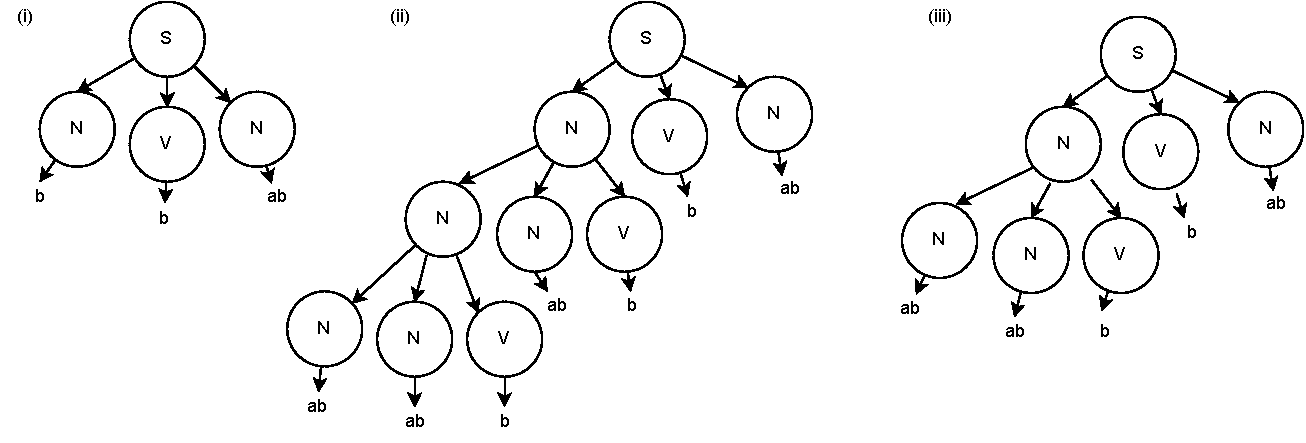
\includegraphics[width = \textwidth]{ex5a.pdf}
\end{figure}

\paragraph*{(b)} \(G\) is ambiguous because there exists \(w \in L(G)\) that has two parse trees. Consider \(w = abbbbb \in L(G)\). The following two parse trees generate the same string \(abbbbb\).
\begin{figure}[htp!]
  \centering
  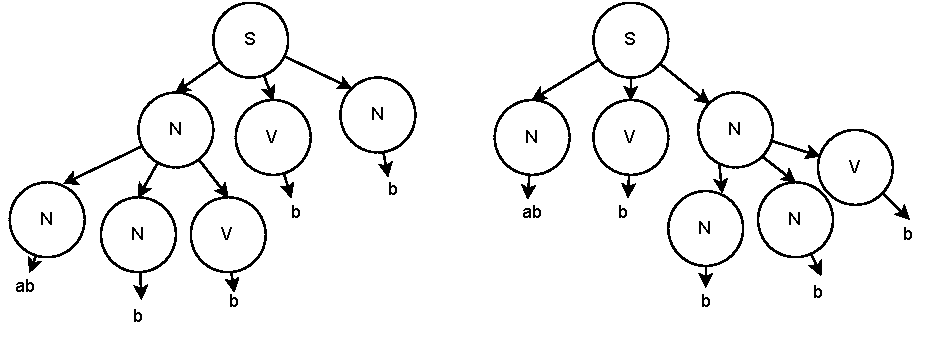
\includegraphics[scale = 0.8]{ex5b.pdf}
\end{figure}

\paragraph*{(c)} \(G' = (\{S, A, V, N\}, \{a, b\}, S, P)\) where \(P\) is defined by the following productions:
\begin{align*}
  S &\to AVN\\
  A &\to ANV \mid ab \mid a\\
  N &\to NNV \mid ab \mid b\\
  V &\to b
\end{align*}
\end{document}